%!TEX root = ../main.tex 

\section{Quels sont les types de régulateurs?}


\begin{frame}{DC-DC - Régulateurs Linéaires vs Switching}
\renewcommand{\arraystretch}{1.4}
\begin{table}
    \centering
    \begin{tabular}{>{\color{UDSgreenSolidarite}}c c | c | c}
        \rowcolor{UDSgreenSolidarite}
        \color{white}\textbf{\faList} & \color{white}\textbf{Critère} & 
        \color{white}\textbf{Régulateur Linéaire} & 
        \color{white}\textbf{Régulateur Switching} \\
        \faDollarSign\ & \textbf{Coût}       
            & {\color{UDSgreenFierte}Faible \cmark} 
            & {\color{red}Moyen à Élevé \xmark} \\
        \faPuzzlePiece\ & \textbf{Complexité} 
            & {\color{UDSgreenFierte}Faible \cmark} 
            & {\color{red}Moyen à Élevé \xmark} \\
        \faWaveSquare\ & \textbf{Bruit}      
            & {\color{UDSgreenFierte}Faible \cmark} 
            & {\color{red}Moyen à Élevé \xmark} \\
        \faPercent\ & \textbf{Efficacité} 
            & {\color{red}Faible \xmark} 
            & {\color{UDSgreenFierte}Très Efficace \cmark} \\
        \faRandom\ & \textbf{\boldmath$V_{out}$} 
            & {\color{red}$V_{out} < V_{in}$ \xmark} 
            & {\color{UDSgreenFierte}$V_{out} \subseteq \mathbb{R}$ \cmark} \\
        \faUnlink\ & \textbf{Isolation} 
            & {\color{red} Non \xmark} 
            & {\color{UDSgreenFierte} Possible \cmark} \\
        \faThermometerHalf\ & \textbf{Température}        
            & {\color{red}Élevée \xmark}            
            & {\color{UDSgreenFierte}Faible à Moyenne \cmark} \\
        \faBolt\ & \textbf{Courant}            
            & {\color{red}Faible à Moyen \xmark}
            & {\color{UDSgreenFierte}Moyen à Élevé \cmark} \\
    \end{tabular}
\end{table}
\end{frame}

\subsection{Régulateurs Linéaires}


\begin{frame}{Régulateur Linéaire (LDO) - Résumé}
    \begin{columns}
        \begin{column}{0.5\textwidth}
            \vspace{-24pt}
            \begin{itemize}
                \item<1-> Régulateur très simple
                \begin{itemize}
                    \item<1-> IC
                    \item<1-> Pièces autours
                \end{itemize}
                \item<2-> Output très stable
                \begin{itemize}
                    \item<2-> PSRR
                \end{itemize}
                \item<3-> $V_{in} - \SI{0.3}{\volt} > V_{out}$
                \item<3-> Isolation impossible
                \item<4-> Très peu efficace
                \begin{itemize}
                    \setlength{\itemsep}{4pt}
                    \item<4-> $I_{in} = I_{out}$
                    \item<4-> $\eta = \dfrac{P_{out}}{P_{in}} = \dfrac{V_{out}}{V_{in}}$
                \end{itemize}
                \item<5-> Power dissipée en chaleur!
                \item<5-> Limite le courant
            \end{itemize}
        \end{column}

        \begin{column}{0.5\textwidth}
            \renewcommand{\arraystretch}{1.4}
            \begin{table}
            \centering
            \begin{tabular}{>{\color{UDSgreenSolidarite}}c | c}
                \rowcolor{UDSgreenSolidarite}
                \color{white}\textbf{\faList} & \color{white}\textbf{Régulateur Linéaire}\\
                \faDollarSign\ & {\color{UDSgreenFierte}Faible \cmark}\\
                \faPuzzlePiece\ & {\color{UDSgreenFierte}Faible \cmark}\\
                \ifnum\slideno>1
                \faWaveSquare\ & {\color{UDSgreenFierte}Faible \cmark}\\
                \ifnum\slideno>2 
                \faRandom\ & {\color{red}$V_{out} < V_{in}$ \xmark}\\
                \faUnlink\ & {\color{red}Non \xmark}\\
                \ifnum\slideno>3 
                \faPercent\ & {\color{red}Faible \xmark}\\
                \ifnum\slideno>4 
                \faThermometerHalf\ & {\color{red}Élevée \xmark}\\
                \faBolt\ & {\color{red}Faible à Moyen \xmark}\\
                \fi\fi\fi\fi
            \end{tabular}
            \end{table}
            \vfill
            \begin{figure}
                \centering
                \includegraphics<-2>[width=0.33\textwidth]{pictures/linear-regulator-7805.png}
            \end{figure}
        \end{column}
    \end{columns}
\end{frame}


\begin{frame}{Régulateur Linéaire - Fonctionnement}
    \begin{center}
        \resizebox{\textwidth}{!}{
        \begin{circuitikz}[american voltages]
            \draw [thick]
            (22, 8) to [european resistor, l=${LOAD}$] (22, 0) node [ground] {}
            (20.5, 8) to [C] (20.5, 0) node [ground]{}
            (0, 8) to [C] (0, 0) node [ground]{};
            \draw
            (0, 8) node [vcc, xscale=1.5, yscale=1.5] {$V_{in}$};
                
            % Feedback Voltage Divider
            \only<-2> {
                \draw [thick]
                (17, 8) to [R] (17, 4) to [R] (17, 0) node[ground] {};
            }
            \only<3-> {
                \draw [thick]
                (17, 8) to [R] (17, 4) to [R, v^=\LARGE{$V_{fb}$}] (17, 0) node[ground] {};
            }

            % Zener Voltage Reference
            \only<1> {
                \draw [thick]
                (5.5, 0) node[ground]{} to [empty ZZener diode] (5.5, 5) to [R] (5.5, 8);
            }
            \only<2-> {
                \draw [thick]
                (5.5, 0) node[ground]{} to [empty ZZener diode, v^<={\LARGE $V_{ref}$}] (5.5, 5) to [R, f<^={\LARGE $i_Q$}] (5.5, 8);
            }


            % Comparison OpAmp
            \draw [thick]
            (10, 4) node[op amp, xscale=1.5, yscale=-1.5] (amp) {}
            (amp.+) to [short, -*] (amp.+ -| 5.5, 0)
            (amp.-) to [short] (amp.- -| 7, 0)
            to [short] (7, 1) to [short] (16, 1)
            to [short] (16, 4) to [short, -*] (17, 4);

            % PMOS
            \draw [thick]
            (14, 8) node[pigfete, bodydiode, rotate=90, xscale=2, yscale=-2] (fet) {}
            (fet.G) node [anchor=south, xshift=8pt] {G}
            (fet.D) node [anchor=west, yshift=8pt] {D}
            (fet.S) node [anchor=east, yshift=8pt] {S}
            (fet.G) to [short] (fet.G |- 0, 4) to [short] (amp.out) 
            (fet.D) to [short] (0, 8)
            (fet.S) to (22, 8);

            % Soft-Start Capacitor
            \only<4-> {
                \draw [thick]
                (amp.+ -| 5.5, 0)
                to [short] (amp.+ -| 1.75, 0)
                to [C, l_={\LARGE $C_{SS}$}, color=red] (1.75, 0) node [ground] {};
            }

            % Box
            \only<-4> {
                \draw[dashed, ultra thick, rounded corners] (3, 9.5) rectangle (19, -1.5);
            }


            % Arrows
            \only<2> {
                \draw[->, thick, red] 
                (3.75, 7) to[out=-90, in=90] (3.75, 1);
            }
            \only<3> {
                \draw[->, thick, red] 
                (16.5, 4.5) to[in=0, out=180] (11, 1.5);
            }
            \only<4> {
                \draw[->, thick, red] 
                (4.75, 7.5) to[in=0, out=-90] (2.5, 5.5)
                to[in=90, out=180] (1, 3.5);
            }

        \end{circuitikz}
        }
    \end{center}  
\end{frame}

\begin{frame}{Power Supply Ripple Reduction}
    \begin{columns}
        \begin{column}{0.4\textwidth}
            \begin{center}
                $PSRR = \dfrac{\Delta V_{in}}{\Delta V_{out}}$
            \end{center}
        \end{column}
        \begin{column}{0.5\textwidth}
            \begin{center}
                $PSRR (dB) = -20 \log \left(\dfrac{\Delta V_{in}}{\Delta V_{out}}\right)$
            \end{center}
        \end{column}
    \end{columns}
    \vfill
    \begin{columns}
        \begin{column}{0.3\textwidth}
            \begin{itemize}
                \item Réduction du bruit
                \item À une fréquence
            \end{itemize}
            \pause
            \vspace{12pt}
            \begin{itemize}
                \item Graphique PSRR
                \item Dépend du courant
            \end{itemize}
        \end{column}
        \begin{column}{0.66\textwidth}
            \begin{figure}
                \centering
                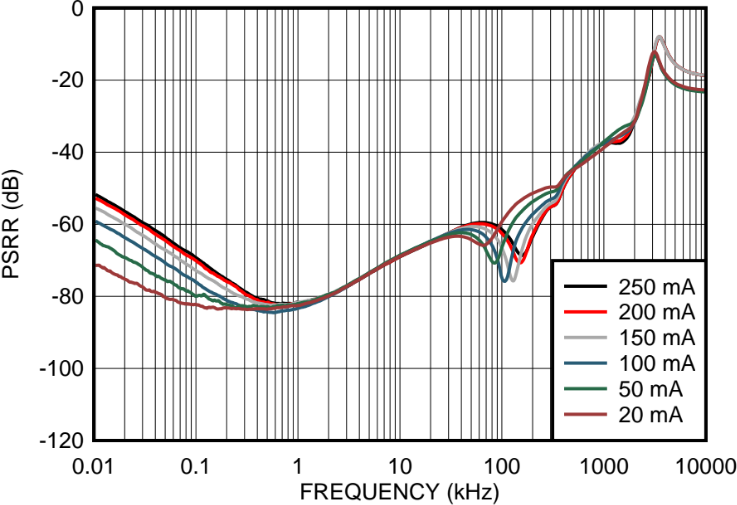
\includegraphics[width=\textwidth, height=0.6\textheight, keepaspectratio]{pictures/psrr-graph.png}
            \end{figure}
        \end{column}
    \end{columns}
\end{frame}

\begin{frame}{Quand choisir un régulateur linéaire?}
\Large
\centering
\begin{tabular}{c l}
    \textcolor{UDSgreenFierte}{\faDollarSign}   & Low-Cost \\
    [0.6em]
    \textcolor{UDSgreenFierte}{\faBolt}         & Peu de courant \\
    [0.6em]
    \textcolor{UDSgreenFierte}{\faCompress}     & Peu d'espace \\
    [0.6em]
    \textcolor{UDSgreenFierte}{\faWaveSquare}   & Bruit très important \\
    [0.6em]
    \textcolor{UDSgreenFierte}{\faPercent}      & Efficacité peu importante \\
    [1.2em]
    \textcolor{UDSgreenFierte}{\faLightbulb}    & Utiliser avec des régulateurs switching!
\end{tabular}
\end{frame}



\subsection{Régulateurs \textit{Switching}}

\begin{frame}{Régulateur Switching - Résumé}
    \begin{columns}
        \begin{column}{0.6\textwidth}
            \vspace{-12pt}
            \begin{itemize}
                \item<1-> Régulateur plus complexe
                \begin{itemize}
                    \item<1-> IC
                    \item<1-> Condensateurs \& bobines
                    \item<1-> Transistors et diodes
                \end{itemize}
                \item<1-> Topologies
                \item<2-> Rajoute du bruit au circuit
                \begin{itemize}
                    \item<2-> Fréquence de \textit{switching}
                \end{itemize}
                \item<3-> Output très grande selon topologie
                \begin{itemize}
                    \item<3-> $V_{out} > V_{in}$
                    \item<3-> $V_{out} < \SI{0}{\volt}$
                    \only<3>{\item \textit{Sortie isolée possible}}
                \end{itemize}
                \item<4-> Extrèmement efficace
                \begin{itemize}
                    \item<4-> 80\% - 90\%
                    \only<4>{\item \textit{Courant \& Tension scale selon demande}}
                \end{itemize}
                \only<5-> {
                \item Bonne gestion thermique
                \begin{itemize}
                    \item Selon topologie
                \end{itemize}
                \item Gros courants
                }
            \end{itemize}
        \end{column}

        \begin{column}{0.4\textwidth}
            \renewcommand{\arraystretch}{1.4}
            \begin{table}
            \centering
            \begin{tabular}{>{\color{UDSgreenSolidarite}}c | c}
                \rowcolor{UDSgreenSolidarite}
                \color{white}\textbf{\faList} & \color{white}\textbf{Régulateur Linéaire}\\
                \faDollarSign\ & {\color{red}Moyen à Élevé \xmark}\\
                \faPuzzlePiece\ & {\color{red}Moyen à Élevé \xmark}\\
                \ifnum\slideno>1
                \faWaveSquare\ & {\color{red}Moyen à Élevé \xmark}\\
                \ifnum\slideno>2 
                \faRandom\ & {\color{UDSgreenFierte}$V_{out} \subseteq \mathbb{R}$ \cmark}\\
                \faUnlink & {\color{UDSgreenFierte}Possible  \cmark}\\
                \ifnum\slideno>3 
                \faPercent\ & {\color{UDSgreenFierte}Très Efficace \cmark}\\
                \ifnum\slideno>4 
                \faThermometerHalf\ & {\color{UDSgreenFierte}Faible à Moyenne \cmark}\\
                \faBolt\ & {\color{UDSgreenFierte}Moyen à Élevé \cmark}\\
                \fi\fi\fi\fi
            \end{tabular}
            \end{table}
            \vfill
            \begin{figure}
                \centering
                \includegraphics<-3>[width=0.5\textwidth]{pictures/switching-regulator-ic.png}
            \end{figure}
        \end{column}
    \end{columns}
\end{frame}

\begin{frame}{Topologies de Régulateurs Switching}
    \centering
    \Large
    \renewcommand{\arraystretch}{1.5}
    \begin{tabular}{>{\color{UDSgreenFierte}}c l | c | c}
        \rowcolor{UDSgreenSolidarite}
        & \textcolor{white}{\textbf{Topologie}} & 
        \textcolor{white}{\boldmath$V_{out}$} & 
        \textcolor{white}{\textbf{Isolation}} \\

        \faArrowDown   & \textbf{Buck}        & $V_{out} < V_{in}$                            & \xmark \\
        \faArrowUp     & \textbf{Boost}       & $V_{out} > V_{in}$                            & \xmark \\
        \faArrowsAltV  & \textbf{Buck-Boost}  & $V_{out} \subseteq \mathbb{R}$ & \xmark \\
        \faRetweet     & \textbf{SEPIC}       & $V_{out} \ge \SI{0}{\volt}$ & \xmark \\
        \faBorderStyle & \textbf{Flyback}     & $V_{out} \subseteq \mathbb{R}$ & \cmark
    \end{tabular}
\end{frame}

\begin{frame}{Régulateur Switching - Principe principal}
    \begin{itemize}
        \item Une bobine s'oppose aux changements de courant
    \end{itemize}

    \vfill
    \begin{figure}
        \centering
        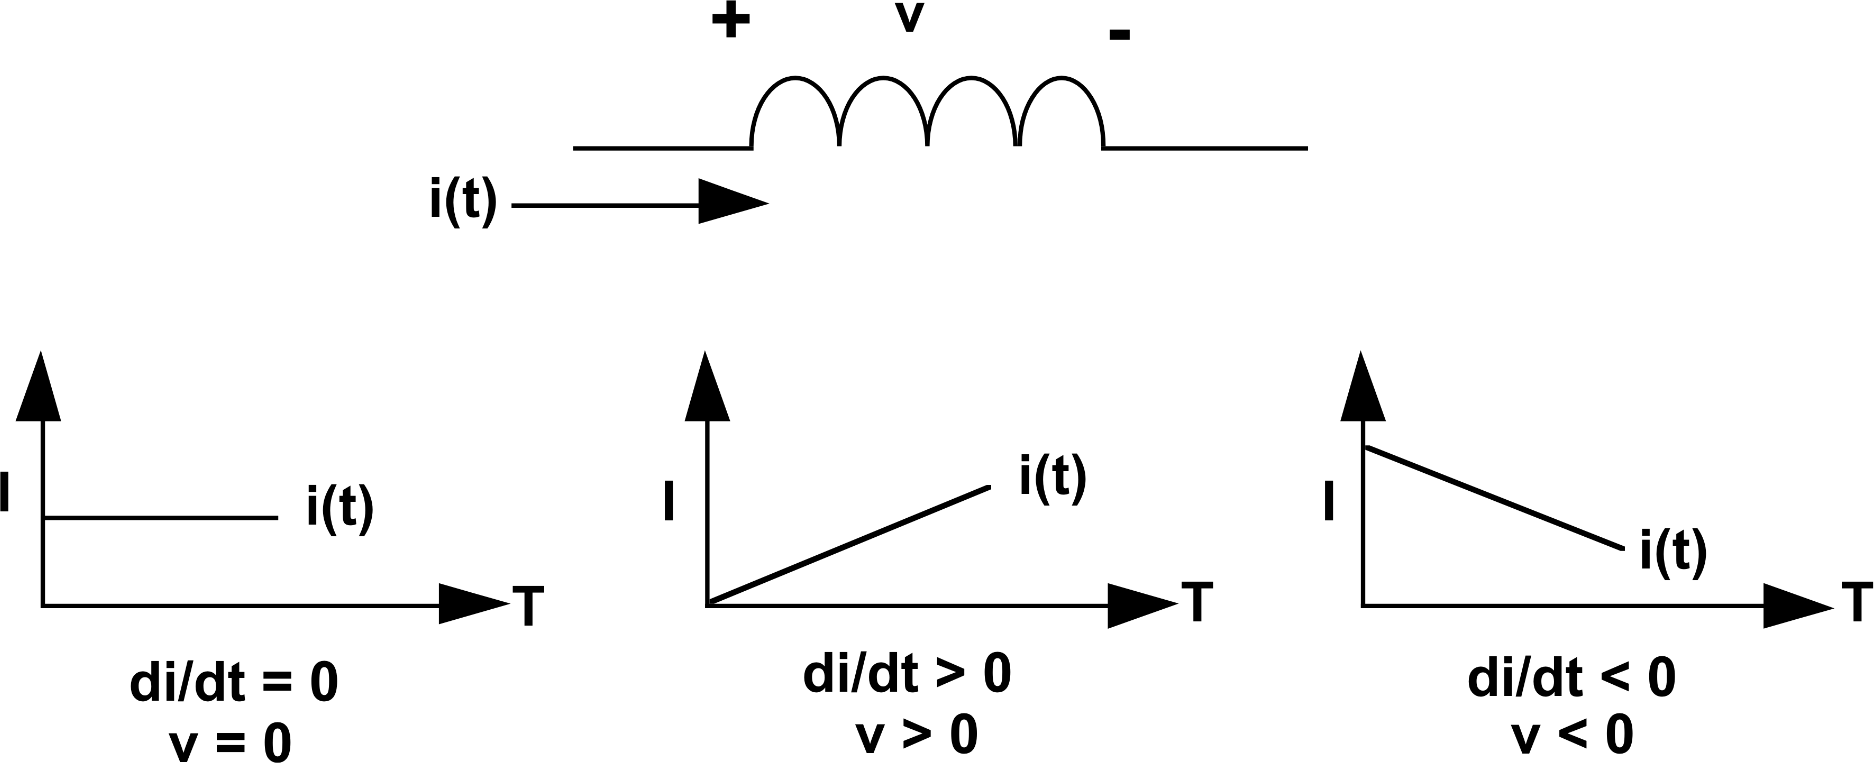
\includegraphics[width=\textwidth]{pictures/law-of-inductance.png}
    \end{figure}
\end{frame}

\begin{frame}{Régulateur Switching - Buck - Fonctionnement}
    \centering
    \resizebox{\textwidth}{!}{
    \ctikzset{inductors/scale=2}
    \begin{circuitikz}[american voltages,
        block/.style = {rectangle, draw, minimum height=1cm,        minimum width=2.5cm, align=center},
        node distance=0.8cm and 0.6cm,
        >={Stealth[round]}
    ]
        \draw [thick]
        (22, 8) to [european resistor, l=${LOAD}$] (22, 0) node [ground] {}
        (19.5, 8) to [C] (19.5, 0) node [ground]{}
        (0, 8) to [C] (0, 0) node [ground]{};
        \draw
        (0, 8) node [vcc, xscale=1.5, yscale=1.5] {$V_{in}$};


        % PMOS
        \only<1> {
            \draw [thick]
            (6, 8) node[pigfete, bodydiode, rotate=90, xscale=2, yscale=-2] (fet) {};
        }
        \only<2> {
            \draw [thick]
            (6, 8) node[pigfete, bodydiode, rotate=90, xscale=2, yscale=-2, color=UDSgreenFierte] (fet) {};
        }
        \only<3> {
            \draw [thick]
            (6, 8) node[pigfete, bodydiode, rotate=90, xscale=2, yscale=-2, color=red] (fet) {};
        }

        \draw [thick]
        (fet.G) node [anchor=south, xshift=8pt] {G}
        (fet.D) node [anchor=west, yshift=8pt] {D}
        (fet.S) node [anchor=east, yshift=8pt] {S}
        (fet.D) to [short] (0, 8);

        \only<1> {
            \draw[thick]
            (fet.S) to [short] (12, 8) to [american inductor] (20, 8) to [short] (22, 8);
        }
        \only<2-> {
            \draw[thick]
            (fet.S) to [short] (12, 8) to [american inductor, f>^={\Large$i$}] (20, 8) to [short] (22, 8);
        }

        % Control Block
        \draw [thick]
        (fet.G |- 0, 4) node [block, anchor=south, yshift=-8pt] (control) {\LARGE Control}
        (control.north) to [short] (fet.G);

        % Schottky Diode
        \draw [thick]
        (12, 0) node[ground]{} to [empty Schottky diode] (12, 8);


        % Arrows
        \only<2> {
            \draw[->, ultra thick, red] 
            (4, 9.5) to[out=0, in=180] (8, 9.5);
            \draw[->, ultra thick, red] 
            (12.5, 9.5) to[out=0, in=180] (17, 9.5);
            \draw[->, ultra thick, red] 
            (19.5, 9.5) to[out=0, in=90] (21, 5);

            \draw[->, ultra thick, red] 
            (21, 3) to[out=-90, in=0] (19.5, -1);
            \draw[->, ultra thick, red] 
            (16, -1) to[out=180, in=0] (13, -1);
            \draw[->, ultra thick, red] 
            (9, -1) to[out=180, in=0] (5, -1);
            \draw[->, ultra thick, red] 
            (2.5, 1.5) to[out=120, in=240] (2.5, 6.5);
        }
        \only<3> {
            \draw[->, ultra thick, red] 
            (12.5, 5.5) to[out=90, in=180] (14.5, 7.5)
            to [out=0, in=180] (16.5, 7.5)
            to [out=0, in=90] (18.75, 5);
            \draw[->, ultra thick, red] 
            (18.75, 2) to[out=-90, in=0] (16.5, 0.5)
            to [out=180, in=0] (14.5, 0.5)
            to [out=180, in=-90] (12.5, 2.5);

            \draw[->, ultra thick, red] 
            (19.75, 6.5) to[out=90, in=180] (20.75, 7.5)
            to[out=0, in=90] (21.75, 6.5);
            \draw[->, ultra thick, red] 
            (21.75, 1.5) to[out=-90, in=0] (20.75, 0.5)
            to[out=180, in=-90] (19.75, 1.5);
        }
    \end{circuitikz}
    }
\end{frame}

\begin{frame}{Régulateur Switching - Buck - Waveform}
   \large
    \renewcommand{\arraystretch}{1.25}
    \begin{tabular}{>{\color{UDSgreenFierte}}c l}
        \faToggleOn   & \color{black} Le courant augmente tranquillement \\
        \color{red}\faToggleOff & \color{black} Le courant descend \\
        \faRetweet    & \color{black} Il y a toujours du courant qui s'en va vers la load \\
        \hspace{12pt}\color{red}\faBan & \hspace{12pt}\color{black} Il n'y a pas toujours du courant qui sort de la source \\
        \hspace{12pt}\faChartLine & \hspace{12pt}\color{black} $I_{out} > I_{in}$ \\
    \end{tabular}

    \vfill
    \begin{figure}
        \centering
        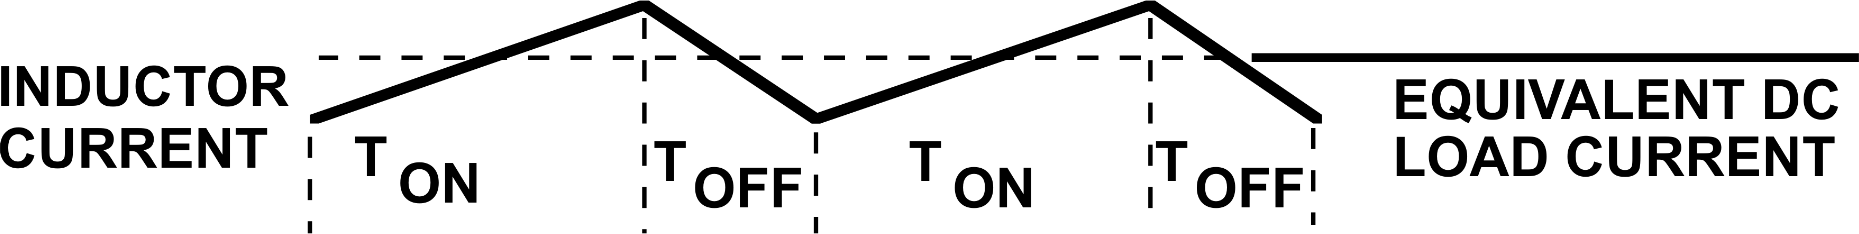
\includegraphics[width=\textwidth]{pictures/buck-switching-current.png}
    \end{figure}
\end{frame}

\begin{frame}{Régulateur Switching - Buck - Waveform}
    \vfill
    \begin{figure}
        \centering
        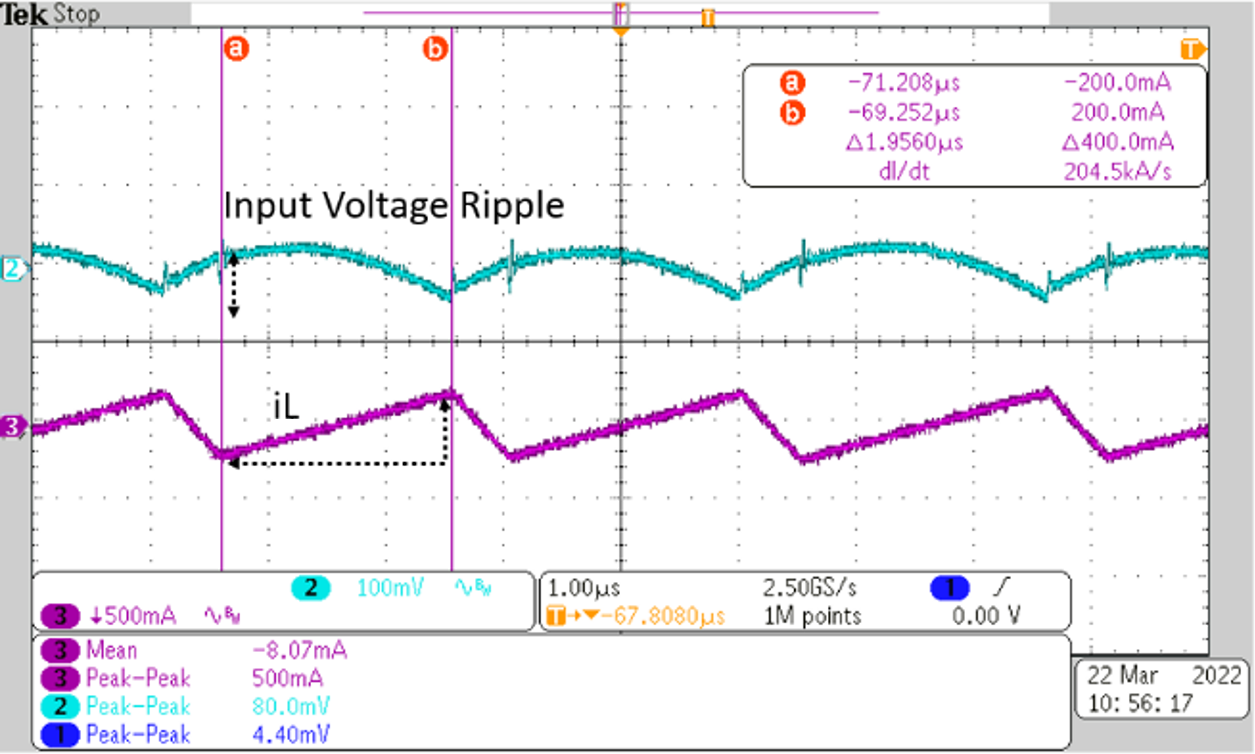
\includegraphics[width=\textwidth, height=0.8\textheight, keepaspectratio]{pictures/buck-switching-output.png}
    \end{figure}
\end{frame}


\begin{frame}{Régulateur Switching - Boost - Fonctionnement}
    \centering
    \resizebox{\textwidth}{!}{
    \ctikzset{inductors/scale=2}
    \begin{circuitikz}[american voltages,
        block/.style = {rectangle, draw, minimum height=1cm, minimum width=2.5cm, align=center},
        node distance=0.8cm and 0.8cm,
        >={Stealth[round]}
    ]
        \draw [thick]
        (22, 8) to [european resistor, l=${LOAD}$] (22, 0) node [ground] {}
        (19.5, 8) to [C] (19.5, 0) node [ground]{}
        (0, 8) to [C] (0, 0) node [ground]{};
        \draw
        (0, 8) node [vcc, xscale=1.5, yscale=1.5] {$V_{in}$};


        % PMOS
        \only<1> {
            \draw [thick]
            (10, 4) node[nigfete, bodydiode, xscale=2, yscale=2] (fet) {};
        }
        \only<2> {
            \draw [thick]
            (10, 4) node[nigfete, bodydiode, xscale=2, yscale=2, color=UDSgreenFierte] (fet) {};
        }
        \only<3> {
            \draw [thick]
            (10, 4) node[nigfete, bodydiode, xscale=2, yscale=2, color=red] (fet) {};
        }

        \draw [thick]
        (fet.G) node [anchor=south, xshift=8pt] {G}
        (fet.D) node [anchor=west, yshift=8pt] {D}
        (fet.S) node [anchor=east, yshift=8pt] {S}
        (fet.D) to [short] (fet.D |- 0, 8)
        (fet.S) to [short] (fet.S |- 0, 0) node [ground] {};

        % Control Block
        \draw [thick]
        (fet.G -| 3.5, 4) node [block, anchor=west] (control) {\LARGE Control}
        (control.east) to [short] (fet.G);

        % Inductor
        \only<1> {
            \draw [thick]
            (0, 8) to [american inductor] (fet.D |- 0, 8);
        }
        \only<2-> {
            \draw [thick]
            (0, 8) to [american inductor, f>^={\Large$i$}] (fet.D |- 0, 8);
        }

        % Diode
        \draw [thick]
        (fet.D |- 0, 8) to [empty Schottky diode] (22, 8);


        % Arrows
        \only<2> {
            \draw[->, ultra thick, red] 
            (0.5, 5.5) to[out=90, in=180] (2.5, 7.5)
            to [out=0, in=180] (6.5, 7.5)
            to [out=0, in=90] (8.75, 5.5);
            \draw[->, ultra thick, red] 
            (8.75, 2) to[out=-90, in=0] (6.5, 0.5)
            to [out=180, in=0] (2.5, 0.5)
            to [out=180, in=-90] (0.5, 2.5);

            \draw[->, ultra thick, red] 
            (19.75, 6.5) to[out=90, in=180] (20.75, 7.5)
            to[out=0, in=90] (21.75, 6.5);
            \draw[->, ultra thick, red] 
            (21.75, 1.5) to[out=-90, in=0] (20.75, 0.5)
            to[out=180, in=-90] (19.75, 1.5);

            \draw[->, line width=4pt, UDSgreenCreativite]
            (11.5, 6) to [out=90, in=90] (11.5, 1);
        }
        \only<3> {
            \draw[->, ultra thick, red] 
            (4, 9.5) to[out=0, in=180] (8, 9.5);
            \draw[->, ultra thick, red] 
            (12.5, 9.5) to[out=0, in=180] (17, 9.5);
            \draw[->, ultra thick, red] 
            (19.5, 9.5) to[out=0, in=90] (21, 5);

            \draw[->, ultra thick, red] 
            (21, 3) to[out=-90, in=0] (19.5, -1);
            \draw[->, ultra thick, red] 
            (16, -1) to[out=180, in=0] (13, -1);
            \draw[->, ultra thick, red] 
            (9, -1) to[out=180, in=0] (5, -1);
            \draw[->, ultra thick, red] 
            (2.5, 1.5) to[out=120, in=240] (2.5, 6.5);
        }
        \only<2-> {
            \draw[->, line width=4pt, UDSgreenCreativite]
            (3, 9) to [out=0, in=180] (8, 9);
        }
    \end{circuitikz}
    }
\end{frame}